%% LyX 2.2.3 created this file.  For more info, see http://www.lyx.org/.
%% Do not edit unless you really know what you are doing.
\documentclass[oneside,italian]{book}
\usepackage[T1]{fontenc}
\usepackage[latin9]{inputenc}
\usepackage{geometry}
\geometry{verbose,tmargin=2.5cm,bmargin=2cm,lmargin=2cm,rmargin=2cm}
\setcounter{secnumdepth}{3}
\setcounter{tocdepth}{3}

\makeatletter
%%%%%%%%%%%%%%%%%%%%%%%%%%%%%% User specified LaTeX commands.
\usepackage{listings,xcolor,courier,bookmark}
\usepackage{listingsutf8}
\definecolor{darkblue}{named}{blue}
\definecolor{darkred}{named}{red}
\definecolor{grau}{named}{gray}
\let\Righttorque\relax
\lstset{
captionpos=b,
commentstyle=\color[rgb]{0.133,0.545,0.133},
keywordstyle=\color{darkblue},
stringstyle=\color{darkred},
extendedchars=true,
basicstyle=\small\ttfamily,
showstringspaces=false,
tabsize=2,
numbers=left,
numberstyle=\tiny,
breakautoindent  = true,
breakindent      = 2em,
breaklines       = true,
postbreak        = ,
prebreak         = \raisebox{-.8ex}[0ex][0ex]{\Righttorque},
showspaces=false, 
showtabs=false, 
showstringspaces=false,
language=VHDL,
frame=single,
morecomment=[s]{--}
}


\renewcommand*{\lstlistingname}{Codice Componente}


\usepackage{fancyhdr}
\pagestyle{fancy}

\fancyhead{} 
\fancyfoot{} 

\fancyhead[RO,LE]{\bfseries \leftmark}
\fancyfoot[LE,RO]{\thepage}
\fancyfoot[LO,CE]{Tesina in ASE: Architetture dei Sistemi di Elaborazione}
\renewcommand{\headrulewidth}{0.4pt}
\renewcommand{\footrulewidth}{0.4pt}

\date{}
\cfoot{}

\makeatother

\usepackage{babel}
\begin{document}

\section{Soluzione}


\subsection{Schematici}

Il seguente circuito implementa l' algortimo RSA per la firma di un
messaggio, applica una funzione di hash sul messaggio e verifica che
il messaggio ricevuto sia coretto.

L' intera procedura � divisa nelle seguenti fasi: 
\begin{itemize}
\item vengono scelti i valori caratteristici per inviare il dato (p pari
a 3, q 11, e 7 e d 3) ed il messaggio da inviare;
\item si applica la funzione di hashing sul messaggio, utilizzando il metodo
della moltiplicazione;
\item viene applicata la firma sul messaggio originale utilizzando la chiave
privata, il trasmettitore invia i due dati appena calcolati (anche
se non � presente un vero e proprio invio essendo trasmettitore e
ricevitore implementati sulla stessa board);
\item Il ricevitore applica la chiave pubblica sul messaggio firmato, ne
effettua l' hashing e verifica se la sua versione del messaggio a
cui � stato applicato l' hashing � identico a quello che � stato ricevuto.
\end{itemize}
Cos� facendo garantiamo sia la segretezza( infatti non mandiamo il
messaggio in chiaro), sia l' autenticazione( chi riceve il messaggio
pu� verificare effettuando l' hashing con parametri convenuti non
� stato modificato),

Di seguito vengono descritte le varie componenti che vengono utilizzate
per effettuare l' hashing e firmare il messaggio.

\subsubsection{Funzione hash}

\begin{figure}[H]
	\centering
	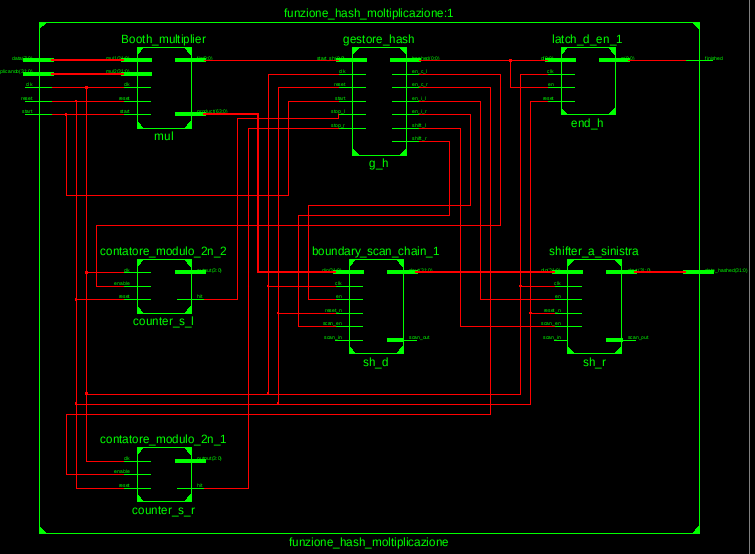
\includegraphics[scale=0.6]{esercizio17/images/hash.png}
	\caption{hasher}
	\label{fig:Mod_exp}
\end{figure}Il circuito � stato realizzato in due differenti modi: 
\begin{itemize}
\item nel primo caso si utilizza una macchina a stati finiti descritta da
cinque stati: 
\begin{itemize}
\item idle, stato di riposo dell' automa; 
\item init in cui si attende che il moltiplicatore termini il suo compito; 
\item shifting\_r in cui il valore della moltiplicazione viene shiftato
a destra; 
\item shifting\_l il valore viene shiftato a sinistra; ended per comunicare
la fine dell' operazione di hash;
\end{itemize}
\item nel secondo si � utilizzato lo stesso procedimento ma il tutto viene
implementato in un process.
\end{itemize}
Viene utilizzata la seconda soluzione perch� occupa meno spazio, dato
che le operazioni di shifting consistono semplicemente, nel caso dello
shifting a destra prendere i sedici bit pi� significativi dal risultato
della moltiplicazione, quando si shifta a sinistra basta accodare
sedici zeri per avere lo stesso risultato della prima soluzione.

Il circito viene cos� descritto poich� tale forma di hashing prevedere
di moltiplicare il dato per un valore A il quale � un numero compreso
tra 0 ed 1, di cui il denominatore � un multiplo di due, per tale
ragione di � scelto di moltiplicare per un valore W ed infine di shiftare
a destra un numero di volte pari al valore dell' esponente, tale numero
� la parte decimale del valore del dato per W (perch� quando shiftiamo
inseriamo degli zero fittizzi), dopodich� si effettua uno shifting
a sinistra di un numero pari di volte affinch� la nostra parte deciamale
rientri nella parte del registro da inviare.

\subsubsection{Esponenziatore}

Per effettuare l' elevazione a potenza con il modulo, ci siamo riferiti
a questo algoritmo :

\begin{figure}[H]
	\centering
	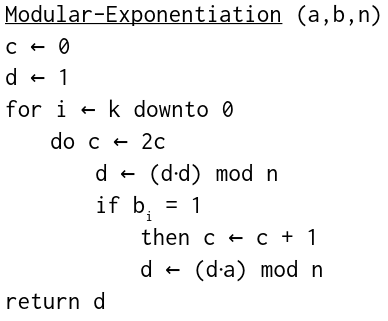
\includegraphics[scale=0.8]{esercizio17/images/mod_exp.png}
	\caption{Algoritmo per modular exponentiational di un messaggio}
	\label{fig:Mod_exp}
\end{figure}

L ' algoritmo cicla sul numero di bit dell ' esponente, moltiplica
il valore d prima per se stesso e ne fa il modulo, questo stesso valore
di d per la base quando il valore dell' esponente in forma binaria
assume valore uno e ne effettua il modulo, (il parametro c non occorre
per il calcolo del valore finale, occorre solo a capire in realt�
alla fine se il numero � stato elevato per il corretto esponente). 

\begin{figure}[H]
	\centering
	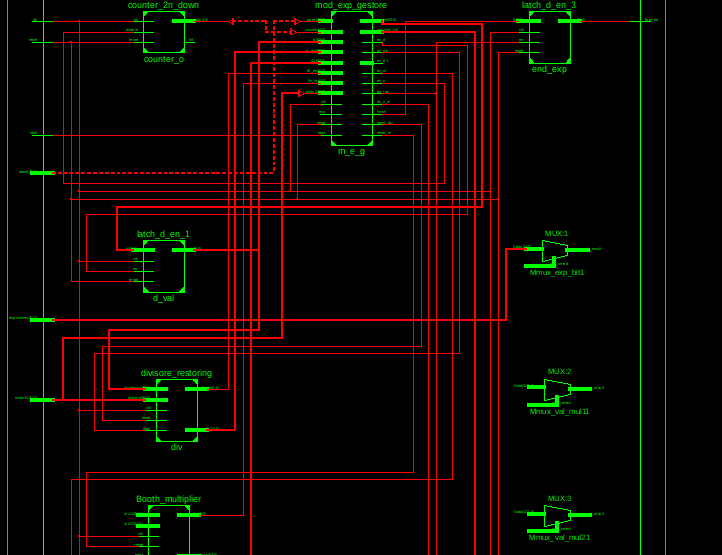
\includegraphics[scale=0.6]{esercizio17/images/exp.png}
	\caption{Hardware Exponentiational}
\end{figure}

Utiliziamo questo algoritmo perch� ci permette di riutilizzare componenti
gi� sviluppati negli esercizi precedenti, difatti osservando lo schematico,
vi � presente un moltiplicatore di Booth e il divisore restoring per
le varie operazioni prodotto e modulo, un contatore down per indicare
quale dei bit dell' esponente dobbiamo analizzare e dei selettori
descritti con il costrutto with select per selezionare quali valori
devono essere moltiplicati. La macchina a stati finiti non fa altro
che eseguire i vari passi dell' algoritmo, per� per problemi relativi
al timing � stata realizzata alla fine con un singolo process, difatti
una prima realizzazione con due process determinava che alcuni registri
contenti i dati dell' operazione assumessero un valore indefinito
(veniva sintetizzata un macchina che doveva avere una frequenza di
clock minore da quella generabile dalla scheda). 

Per problemi di spazio, si � ricorsi a componenti per la moltiplicazione
e divisione seriali, oltre ad riutilizzarli all' interno dello stesso
progetto difatti il moltiplicatore di Booth � stato utilizzato per:
calcolare il prodotto di pq ed l' esponenziazione.

\subsection{Codice}

\href{run:progetti/RSA/RSA.xise}{RSA ISE}


\end{document}
